\chapter{Connell-Hollingsworth Conjecture}\label{c10}

This\pageoriginale lecture continues the discussion of geometric
groups started in Lecture \ref{c9}. 

\begin{defi}\label{c10:defi10.1}
  An automorphism $f: G \to G$ is $\epsilon$-blocked if there exists a
  partition $\mathcal{P}$ of the basis $\{ x_1, \ldots , x_n\}$ for
  the geometric group $G$ such that, for each set $S \in
  \mathcal{P}$, we have
  \begin{enumerate}
    \item diam $S \leq \epsilon$ and
      \item $f (\ob{S}) \subset \ob{S}$ denotes
        the subgroup of $G$ generated by $S$.
  \end{enumerate}
\end{defi}

\begin{lemma}\label{c10:lem10.2}
  If $f$ is $\delta_0/3$-blocked, then $\hat{f}$ represents 0 in $Wh
  (\Gamma)$. 
\end{lemma}

\begin{proof}
  Pick a base point $*_\mathcal{S}$ for each partition set
  $\mathcal{S} \in \mathcal{P}$ from among the elements $x_j \in
  \mathcal{S}$, and pick paths $\alpha_{\mathcal{S}}$ aonnecting $*$
  to $*_{\mathcal{S}}$. For each $x_i \in \mathcal{S}$ pick a path
  $\ob{\alpha}_i$  connecting $*_{\mathcal{S}}$ to $x_i$ such that
  $diam \ob{\alpha_i} \leq \delta_1$. Let $\alpha_i = \ob{\alpha}_i =
  \ob{\alpha_i}* \alpha_{\mathcal{S}}$. Then the loops $\alpha_i^{-1}
  * \gamma_{ij}* \alpha_{j}$, such that $f_{ij} \neq 0$, are all
  ineseential as is seen from Figure 8.
  \begin{figure}[H]
    \centering{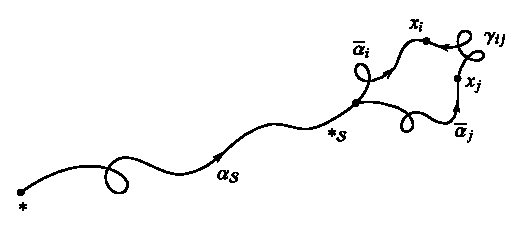
\includegraphics{vol86-figures/fig8.eps}\\
    Figure 8}
  \end{figure}
  Therefore, $\hat{f} = f \in GL_n (\mathbb{Z})$. Hence, its value in
  $Wh(\Gamma)$ is in the image of $Wh (1) = 0$. 
\end{proof}

\begin{remark*}
  Note that the entries of $\hat{f}$, where $f$ is any
  $\delta_0/3$-automor\-phism, are monomials from
  $\mathbb{Z}\Gamma$. The following is an example of a monomial matrix
  which represents a non zero element in $Wh \Gamma$. In this example,
  $\Gamma$ is the cyclic group of order 5 generated by  $x$. 
\end{remark*}

Consider\pageoriginale the unit $1+ x - x^{-3}$ in \text{Units}
$(\mathbb{Z}\Gamma)$. It represents a non-zero element in $Wh\Gamma$
since it is \textit{not} a monimial. But $1+ x- x^{-3}$ is equivalent
to the following $3 \times 3$ matrix 
$$
\begin{pmatrix}
  1+ x- x^{3} & 0 & 0\\
  0 & 1 & 0\\
  0 & 0 & 1
\end{pmatrix}
$$
by stabilization. This matrix is in turn equivalent to 
$$
A= 
\begin{pmatrix}
  1 & x & x^3\\
  -1 & 1 &0\\
  1 & 0 & 1
\end{pmatrix}
$$
by elementary column operations. Hence $A$ represents a non-zero
element in $Wh \Gamma$ and the entries in $A$ are all monomial. It
appears likely that every element in $Wh \Gamma$ is represented by a
monomial matrix for an arbitrary group $\Gamma$.

\begin{conj}[Connell-Hollingsworth \cite{20}]\label{c10:conj10.3}
  Let $X$ be an $n$-dimensio\-nal finite simiplicial complex. Given
  $\epsilon > 0$, there exists $\delta> 0$ such that the following is
  true. Every $\delta$-automorphism $f: G \to G$ of a geometric group
  on $X$ can be factored
  $$
  f= f_1 \circ f_2 \cdots \circ f_{n+1}
  $$
  as the composite of $n+1$ $\epsilon$-blocked automorphisms.
\end{conj}

\begin{lemma}\label{c10:lem10.4}
  Assume Conjecture \ref{c10:conj10.3} is true and that $X$ is a
  finite simplicial complex. Then there exists $\delta> 0$ such that
  $\hat{f}$ represents 0 in $WH\Gamma$ for any $\delta$-automorphism
  $f:G \to G$ of a geometric group $G$ on $X$.
\end{lemma}

\begin{proof}
  Let $n = \dim X$ and $\epsilon= \delta_0 /6n$. Then $\delta$ is the
  number posited in Conjecture \ref{c10:conj10.3} relative to
  $\epsilon$. (We may assume that $\delta \leq \delta_0/3$.) Express
  $f$ as the composition
  $$
  f=f_1 \circ f_2 \ldots \circ f_{n+1}
  $$
  where each $f_i$ is $\epsilon$-blocked. Note that each $f_i$ is a
  $\delta_0/6n$-automorphism of $G$. Applying Lemma \ref{c9:lem9.3}
  and the remark following it, we obtain
  \begin{equation*}
    \hat{f} = \hat{f}_1 \hat{f}_2 \ldots
    \hat{f}_{n+1}.\tag{1}\label{c10:eq9.3-1} 
  \end{equation*}


But\pageoriginale Lemma \ref{c10:lem10.2} states that each $\hat{f}_i$ represents 0
in $Wh\Gamma$. And equation \eqref{c10:eq9.3-1} implies that the element
in $Wh \Gamma$ represented by $\hat{f}$ is the sum of the elements
represented by $\hat{f}_i$. 
\end{proof}

It is useful to extend the construction $\hat{f}$ and the results
about it to the case of $\delta$-isomorphisms.

\begin{defi}\label{c10:defi10.5}
  A homomorphism $f: G_1 \to G_2$ between two geometric groups on $X$
  is a $\delta$-homomorphism if $\diam f \leq \delta$. It is a
  $\delta$-isomorphism if both $f$ and $f^{-1}$ are $\delta$-homomorphisms.
\end{defi}

If $f$ is a $\delta_0$-homomorphism, then it determines an $m \times
n$ matrix $\hat{f}$ with entries in $\mathbb{Z}\Gamma$ where $m = \rank
G_1$, $n = \rank G_2$. This is done by the natural analogue of the
procedure given in Lecture \ref{c9} for the special case
$G_1=G_2$. But now the construction depends on choices of paths
$\alpha_i$ from $*$ to $x_{i}$ and $\beta_{j}$ from $*$ to $y_j$, 
where $x_1, x_2, \ldots, x_n$ is the
basis for $G_1$ and $y_!, y_2, \ldots y_m$ is the basis for $G_2$. If
we change the choice of these paths, then the following analogue of
Lemma \ref{c9:lem9.2} is true.

\begin{lemma}\label{c10:lem10.6}
  When changes in the choices of the paths $\alpha_i$, $\beta_j$ are
  made, $\hat{f}$ changes to $\mathcal{D} \hat{f} D$ where both
  $\mathcal{D}$ and $D$ are square diagonal matrices whose
  diagonal entries are elements in $\Gamma$.
\end{lemma}

The following analogues of Lemma \ref{c9:lem9.3} and its Corollary
\ref{c9:coro9.4} are also true.

\begin{lemma}\label{c10:lem10.7}
  Suppose $g: G_1 \to G_2$ and $f: G_2 \to G_3$ are both
  $\delta_0/3$-homomorphisms, then $f \circ g$ is a
  $\delta_0$-homomorphism and $\widehat{f \circ g}= \hat{f} \hat{g}$.
\end{lemma}

\begin{coro}\label{c10:coro10.8}
  If $f : G_1 \to G_2$ is a $\delta_0/3$-isomorphism, then $\hat{f}
  \in GL_n (\mathbb{Z}\Gamma)$, where $n= \rank G_1 = \rank G_2$ and
  $\hat{f}$ determines a well defined element in $Wh\Gamma$, which is
  also denoted $\hat{f}$.
\end{coro}

\begin{defi}\label{c10:defi10.9}
  A geometric isomorphism of geometric groups is an isomorphism
  induced by a bijection of their bases.
\end{defi}

\begin{lemma}\label{c10:lem10.10}
  Let\pageoriginale $f: G_1 \to G_2$ be a geometric
  $\delta_0/3$-isomorphism, then $\hat{f}$ represents 0 in $Wh \Gamma$.
\end{lemma}

\begin{proof}
  Note that $\hat{f}$ can be factored as a product of a diagonal
  matrix with diagonal entries in $\Gamma$ and a permutation
  matrix. But both these represent 0 in $Wh\Gamma$. 
\end{proof}

\begin{lemma}\label{c10:lem10.11}
  If two geometric groups $G_1$ and $G_2$ are isomorphic by a
  $\delta$-homomorphism, then they are geometrically
  $\delta$-isomorphic. 
\end{lemma}

\begin{proof}
  Let $x_1, x_2, \ldots , x_n$ and $y_1, y_2, \ldots, y_n$ be the
  bases for the geometric groups $G_1$ and $G_2$. They are also the
  bases for the corresponding \textit{geometric $\mathbb{Q}$-vector
    spaces $G_1 \otimes \mathbb{Q}$} and $G_2 \otimes \mathbb{Q}$. We
  will show, by induction on $n$, that if $G_1 \otimes \mathbb{Q}$ and
  $G_2 \otimes \mathbb{Q}$ are isomorphic via a $\delta$-homomorphism
  $f$, then $G_1$ and $G_2$ are geometrically $\delta$-isomorphic. The
  lemma then follows sicne a $\delta$-homomorphism which induces an
  isomorphism of $G_1$ to $G_2$ induces an isomorphism of $G_1 \otimes
  \mathbb{A}$ to $G_2 \otimes \mathbb{Q}$. Let the $n \times n$ matrix
  $F= (f_{ij})$ be defined by 
  \begin{equation*}
    f(x_j) = \sum_{i} f_{ij}y_i.\tag{1}\label{c10:eq10.11-1}
  \end{equation*}
  Consider the expansion of $\det (F)$ using the last row
  \begin{equation*}
    \det (F) = \sum_i (-1)^{n+j} f_{nj} \det (F^{nj})\tag{2}\label{c10:eq10.11-2}
  \end{equation*}
  where $F^{nj}$ denotes the $(n-1) \times (n-1)$ matrix obtained by
  deleting the last row and $j$-th column from $F$. Since $\det
  (F)\neq 0$, equation \eqref{c10:eq10.11-2} shows that there exists
  an index $j$ such that both
  \begin{equation*}
    f_{nj} \neq 0 ~\text{and}~ \det (F^{nj}) \neq
    0.\tag{3} \label{c10:eq10.11-3}
  \end{equation*}

Now, let $\ob{G}_1$ and $\ob{G}_2$ denote the geometric groups with
bases $x_1, \ldots$, $\hat{x}_j, \ldots, x_n$ and $y_1, y_2, \ldots,
y_{n-1}$, respectively. Using the second assertion in
\eqref{c10:eq10.11-3}, we see that $\ob{G}_1 \otimes \mathbb{Q}$ and
$\ob{G}_2 \otimes \mathbb{Q}$ are isomorphic via a
$\delta$-homomorphism. Hence our inductive assumption yields a
geometric $\delta$-isomorphism $\ob{g}: \ob{G}_1 \to \ob{G}_2$. We
extend $\ob{g}$ to geometric isomorphism $g: G_1 \to
G_2$\pageoriginale by requiring 
$g(x_j)= y_n$. The first assertion in \eqref{c10:eq10.11-3} now shows
that $g$ is a $\delta$-isomorphism.
\end{proof}

\begin{remark*}
  A geometric isomorphism which is a $\delta$-isomorphism is a
  $\delta$-isomorphism. But, an isomorphism which is a
  $\delta$-homomorphism need not be a $\delta$-isomorphism in
  general. To construct an example, consider the matrix identity
  $$
  \begin{pmatrix}
    1 & -1 & 0 & \cdots & 0\\
    0 & 1 & -1 & \ldots & 0\\
    0 & 0 & 1 & \ldots & 0\\
    \cdot & \cdot & \cdot & \cdots & 0\\
    \cdot & \cdot & \cdot & \cdots & 0\\
    \cdot & \cdot & \cdots & 1 & -1\\
    0 & 0 & \cdots & 0 & 1
  \end{pmatrix}^{-1} =
  \begin{pmatrix}
    1 & 1 & \cdot & \cdots & 1\\
    0 & 1 & 1 & \ldots & 1\\
    0 & 0 & 1 & \ldots & 1\\
    \cdot & \cdot & \cdot & \cdots & 1\\
    \cdot & \cdot & \cdot & \cdots & 1\\
    \cdot & \cdot & \cdot & \cdots & 1\\
    0 & 0 & \cdots & 0 & 1    
  \end{pmatrix}
  $$
  We can now prove that following analogue of Lemma \ref{c10:lem10.4}.
\end{remark*}

\begin{lemma}\label{c10:lem10.12}
  Assume that the Conjecture \ref{c10:conj10.3} is true and that $X$
  is a finite simplicial complex. Then there exists $\delta > 0$ such
  that $\hat{f}$ represents 0 in $Wh \Gamma$ for any
  $\delta$-isomorphism $f: G_1 \to G_2$ of geomettric groups on $X$.
\end{lemma}

\begin{proof}
  Denote the nubmer $\delta$ whose existence is posited in Lemma
  \ref{c10:lem10.4} by $\delta_2$. (Recall $\delta_2 \leq
  \delta_0/3$.) Then set $\delta= \delta_2/3$. Let $g: G_2 \to G_1$ be
  the geometric $\delta$-isomorphism given by Lemma
  \ref{c10:lem10.11}. Then the composite $g \circ f: G_1 \to G_1$ is a
  $\delta_2$-isomorphism. Hence, $\widehat{g \circ f}$ represents o in
  $W h \Gamma$, by Lemma \ref{c10:lem10.4}. But $\widehat{g \circ g}=
  \hat{g} \hat{f}$, by Lemma \ref{c10:lem10.7}, and $\hat{g}$
  represents 0 in $Wh\Gamma$, by Lemma
  \ref{c10:lem10.10}. Consequently, $\hat{f}$ also represents
  0. \hfill Q.E.D.
\end{proof}

\begin{remark*}
  The results so far described are due to Connell and Holl\-ings\-worth
  \cite{20}. After proving these, Connell and Hollingsworth then
  proceed to show that the topological in variance of Whitehead
  torisn, first proven by Chapman \cite{18}, would be a consequence of
  Conjecture \ref{c10:conj10.3}. It is also implicit in their paper
  that the controlled (thin) $h$-cobor\-dism, eventually proved by Ferry
  \cite{57}, would also be a consequence of Conjecture
  \ref{c10:conj10.3}. Our next lecture will be devoted to formulating this
  theorem and showing how Conjecture \ref{c10:conj10.3} implies it.
\end{remark*}
